\documentclass[a4paper,11pt]{jsarticle}


% 数式
\usepackage{amsmath,amsfonts}
\usepackage{bm}
% 画像
\usepackage[dvipdfmx]{graphicx}
% 図の先頭につく,fig.1とか図1とか(キャプション)のカスタマイズ
\usepackage{caption}
\captionsetup[figure]{labelformat=simple, labelsep=space, textfont=normalfont, labelfont=bf}
\renewcommand{\figurename}{Fig.}

\begin{document}

\title{進捗報告}
\author{渋谷享史}
\date{\today}
\maketitle
% % 画像挿入
% \begin{figure}[htbp]
%   \vspace{5mm}
%   \center
%   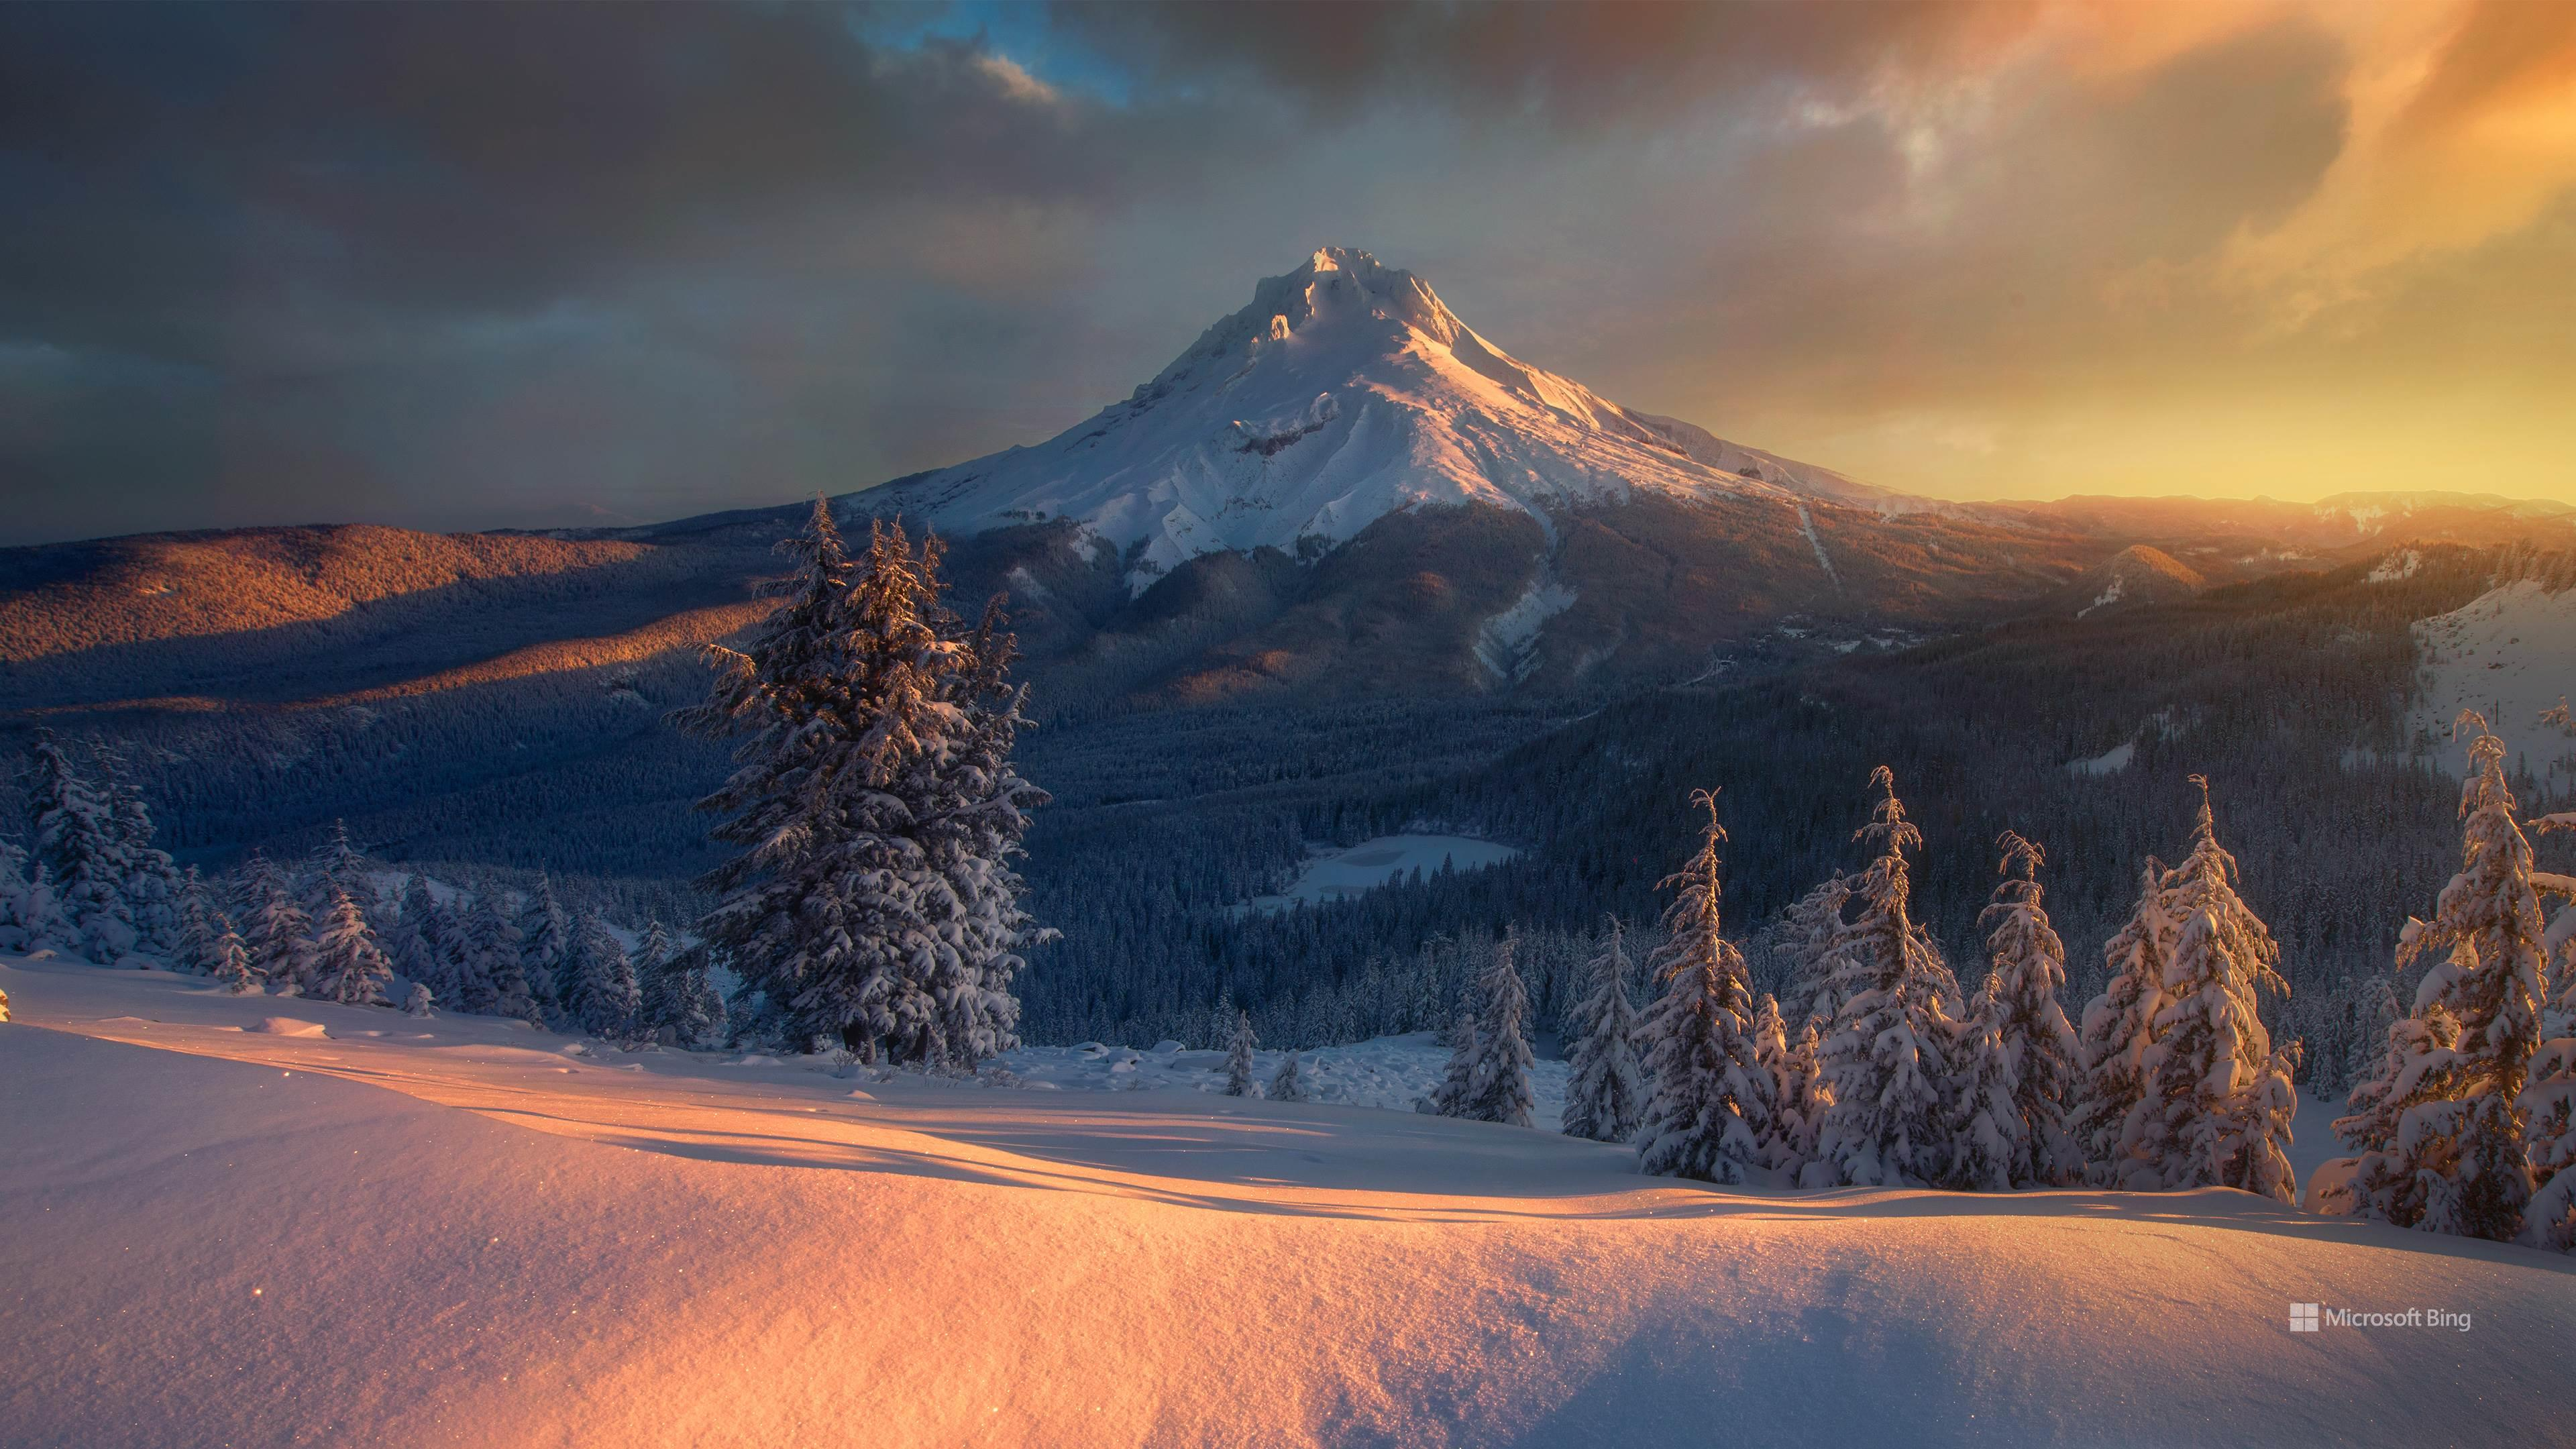
\includegraphics[width=100mm]{images/20240208.jpg}
%   \caption{ブロック図}
%   \label{block}
%   \vspace{5mm}
% \end{figure}
\section{進捗}
\subsection{今回の進捗}
\begin{itemize}
  \item マウスのエンコーダからPI制御で左手法をするプログラムを製作した.
  \item 左手法プログラムの行動を,関数化した
  \item gymのインターフェースについて調べ,MuJoCoの強化学習環境を作成した.
  \item Stable-baseline3を試し,学習を回せることを確認した.
\end{itemize}
\subsection{今後の予定}
\begin{itemize}
  \item 学習のさせ方(報酬設計,どのアルゴリズムを使うか)を決める
  \item プロポーザルを完成させるために,論文の問を考える
  \item オドメトリ値などを状態に含めて学習を行う
\end{itemize}
マウスから取得できる状態をすべて取得できるようにしたので,学習を試してみます.\\
同時に,2輪移動ロボットのプロポーザルを完成させるために,論文を読んで問いを考えます.



\end{document}
